\documentclass{mc2015}

%%%%%%%%%%%%%%%%%%%%%%%%%%%%%%%%%%%%%%%%%%%%%%%%%%%%%%%%%%%%%%%%%%%%%
\usepackage[T1]{fontenc}         % Use T1 encoding instead of OT1
\usepackage[utf8]{inputenc}      % Use UTF8 input encoding
\usepackage{microtype}           % Improve typography
\usepackage{booktabs}            % Publication quality tables
\usepackage{amsmath}
\usepackage{graphicx}
\usepackage{float}
\usepackage[exponent-product=\cdot]{siunitx}
\usepackage[colorlinks,breaklinks]{hyperref}
\hypersetup{linkcolor=black, citecolor=black, urlcolor=black}

\usepackage{lipsum}

\def\equationautorefname{Eq.}
\def\figureautorefname{Fig.}

%%%%%%%%%%%%%%%%%%%%%%%%%%%%%%%%%%%%%%%%%%%%%%%%%%%%%%%%%%%%%%%%%%%%%
% Insert authors' names and short version of title in lines below

\authorHead{Authors' names, use et al. if more than 3}
\shortTitle{Short version of title as entered by author on web page}

%%%%%%%%%%%%%%%%%%%%%%%%%%%%%%%%%%%%%%%%%%%%%%%%%%%%%%%%%%%%%%%%%%%%%
\begin{document}

\title{Title of the paper}

\author{Author A}
\author{Author B\footnote{Footnote, if necessary}}
\affil{Name of Institute \\
  Corresponding Address \\
  A@institute.gov; B@institute.gov}

\author{Author C}
\affil{
  Department of Nuclear Engineering \\
  Name of University \\
  Address \\
  C@name.univ.edu
}

\maketitle

\begin{abstract}
A required 200-250 word abstract starts on this line.  Leave two blank lines before ``ABSTRACT'' and one after.  
Use single (10 point) spacing.  
The abstract is a very brief summary highlighting main accomplishments, what is new, and how it relates to the state-of-the-art.

\emph{Key Words}: List no more than five key words
\end{abstract}

%%%%%%%%%%%%%%%%%%%%%%%%%%%%%%%%%%%%%%%%%%%%%%%%%%%%%%%%%%%%%%%%%%%%%
\section{Introduction}

References can be typeset properly using the provided \textsc{Bib}\TeX style
file. See examples of a journal~\cite{journal}, conference
proceedings~\cite{proceedings}, book~\cite{book}, and
miscellaneous~\cite{misc}.

References to websites are discouraged, but acceptable if absolutely necessary.  It is the author?s responsibility to check links in the pdf file.
Final PDF file size should be no more than 4 MB.  Recommended paper length is 10-12 pages.

\subsection{Second or Subsequent Major Heading}

A logical division of your paper into sections makes it much easier to understand.    

\subsection{Subsection Title: First Character of Each Non-trivial Word is Uppercase}

Equations (Equation \ref{eqn:sample}) should be centered and sequentially numbered to the flush right of the formula.

\begin{equation}
  1+1=2
  \label{eqn:sample}
\end{equation}

\noindent
The continuation of a paragraph after an equation is not indented

\subsubsection{Sub-subsection level and lower: only first character uppercase}

Figures and tables should appear as closely as possible to where they are first cited, e.g. 
Fig. \ref{fig:sample}, in the text.  Figures are numbered in Arabic numerals, with the caption centered below the figure, in boldface. 

\begin{figure}[H]
  \centering
  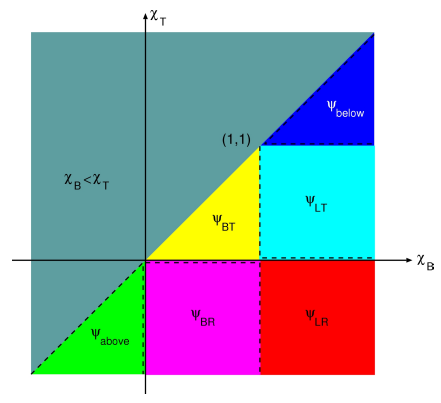
\includegraphics[width=3in]{figure.png}
  \caption{Sample Figure. Color is permitted, but must be readable if printed.}
  \label{fig:sample}
\end{figure}

When importing figures or any graphical image please verify two things:
\begin{enumerate}
\item Any number, text or symbol is no smaller than 10-point after reduction to the actual window in your paper;
\item That it can be translated into PDF.
\end{enumerate}

Tables, like Table \ref{tab:sample}, are numbered in Roman numerals, with the caption centered above the table, in \textbf{boldface}.  
Double-space before and after the table.

\begin{table}
  \centering
  \caption{Sample table: accuracy of nodal and characteristic methods}
  \begin{tabular}{lcccc}
    \toprule
    Mesh & 8 x 8 & 16 x 16 & 32 x 32 & 64 x 64 \\
    \midrule
    Nodal & \num{1.000e-1} & \num{2.500e-2} & \num{6.250e-3} & \num{1.563e-3} \\
    Characteristic & \num{1.000e-1} & \num{2.500e-2} & \num{6.250e-3} & \num{1.563e-3} \\
    \bottomrule
  \end{tabular}
  \label{tab:sample}
\end{table}

%%%%%%%%%%%%%%%%%%%%%%%%%%%%%%%%%%%%%%%%%%%%%%%%%%%%%%%%%%%%%%%%%%%%%
\section{Conclusions}

Present your summary and conclusions here.

%%%%%%%%%%%%%%%%%%%%%%%%%%%%%%%%%%%%%%%%%%%%%%%%%%%%%%%%%%%%%%%%%%%%%
\section{Acknowledgments}

Acknowledge the help of colleagues and sources of funding, as appropriate, including Paul Romano and Tom Sutton, 
who provided this template that is similar to a template from past M\&C meetings.

%%%%%%%%%%%%%%%%%%%%%%%%%%%%%%%%%%%%%%%%%%%%%%%%%%%%%%%%%%%%%%%%%%%%%
\setlength{\baselineskip}{12pt}

\bibliographystyle{mc2015}
\bibliography{references}

%%%%%%%%%%%%%%%%%%%%%%%%%%%%%%%%%%%%%%%%%%%%%%%%%%%%%%%%%%%%%%%%%%%%%
\appendix
\section{}

If necessary, include Appendices numbered in upper case alphabetical order.

In order to ensure a uniform, professional look to the proceedings, please
\emph{\textbf{do not modify}} the format of this template without checking with
the organizers first.

\end{document}
